\documentclass[journal=esthag,manuscript=article]{achemso}
%%%%%%%%%%%%%%%%%%%%%%%%%%%%%%%%%%%%%%%%%%%%%%%%%%%%%%%%%%%%%%%%%%%%%
%% Place any additional packages needed here.  Only include packages
%% which are essential, to avoid problems later. Do NOT use any
%% packages which require e-TeX (for example etoolbox): the e-TeX
%% extensions are not currently available on the ACS conversion
%% servers.
%%%%%%%%%%%%%%%%%%%%%%%%%%%%%%%%%%%%%%%%%%%%%%%%%%%%%%%%%%%%%%%%%%%%%
\usepackage[T1]{fontenc}       % Use modern font encodings
\usepackage[utf8]{inputenc}
\usepackage{amsmath}
\usepackage{enumerate}

% \usepackage{todonotes}

%%%%%%%%%%%%%%%%%%%%%%%%%%%%%%%%%%%%%%%%%%%%%%%%%%%%%%%%%%%%%%%%%%%%%
%% If issues arise when submitting your manuscript, you may want to
%% un-comment the next line.  This provides information on the
%% version of every file you have used.
%%%%%%%%%%%%%%%%%%%%%%%%%%%%%%%%%%%%%%%%%%%%%%%%%%%%%%%%%%%%%%%%%%%%%
%%\listfiles

%%%%%%%%%%%%%%%%%%%%%%%%%%%%%%%%%%%%%%%%%%%%%%%%%%%%%%%%%%%%%%%%%%%%%
%% Place any additional macros here.  Please use \newcommand* where
%% possible, and avoid layout-changing macros (which are not used
%% when typesetting).
%%%%%%%%%%%%%%%%%%%%%%%%%%%%%%%%%%%%%%%%%%%%%%%%%%%%%%%%%%%%%%%%%%%%%
%% \newcommand*\mycommand[1]{\texttt{\emph{#1}}}


%%%%%%%%%%%%%%%%%%%%%%%%%%%%%%%%%%%%%%%%%%%%%%%%%%%%%%%%%%%%%%%%%%%%%
\author{Eduard Szöcs}
\affiliation[Institute for Environmental Sciences]{Institute for Environmental Sciences, University of Koblenz-Landau, Germany}
\email{szoecs@uni-landau.de}
\phone{+49 (0)6341 280 31552}

\author{Marvin Brinke}
\affiliation[German Federal Institute of Hydrology]{German Federal Institute of Hydrology (BfG), Koblenz, Germany}

\author{Bilgin Karaoglan}
\affiliation[German Federal Environmental Agency]{Federal Environmental Agency (UBA), Dessau-Roßlau, Germany}

\author{Ralf B. Schäfer}
\affiliation[University Koblenz-Landau]{Institute for Environmental Sciences, University of Koblenz-Landau, Germany}


%%%%%%%%%%%%%%%%%%%%%%%%%%%%%%%%%%%%%%%%%%%%%%%%%%%%%%%%%%%%%%%%%%%%%
\title[Pesticides small streams]{Pesticides in small streams in Germany}
% \abbreviations{mo, neon, ra, tu, fw}
\keywords{Monitoring, Neonicotinoid, Risk Assessment Toxic Units, Freshwater}
% RAC, 

%%%%%%%%%%%%%%%%%%%%%%%%%%%%%%%%%%%%%%%%%%%%%%%%%%%%%%%%%%%%%%%%%%%%%
\begin{document}
%%%%%%%%%%%%%%%%%%%%%%%%%%%%%%%%%%%%%%%%%%%%%%%%%%%%%%%%%%%%%%%%%%%%%
%% The "tocentry" environment can be used to create an entry for the
%% graphical table of contents. It is given here as some journals
%% require that it is printed as part of the abstract page. It will
%% be automatically moved as appropriate.
%%%%%%%%%%%%%%%%%%%%%%%%%%%%%%%%%%%%%%%%%%%%%%%%%%%%%%%%%%%%%%%%%%%%%
\begin{tocentry}

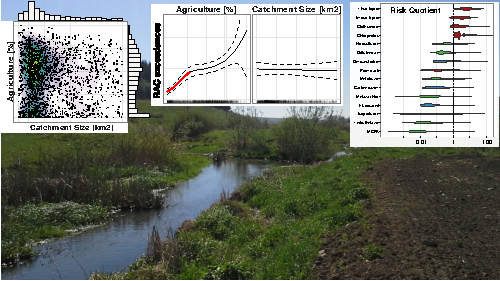
\includegraphics[width=0.7\textwidth]{abstract.pdf}

\end{tocentry}


%%%%%%%%%%%%%%%%%%%%%%%%%%%%%%%%%%%%%%%%%%%%%%%%%%%%%%%%%%%%%%%%%%%%%
\begin{abstract}
% 150-200 words
Small streams are important refugia for biodiversity.
In agricultural areas, they may be at high risk from pesticides that enter streams during rainfall. 
However, most related studies have been limited to a few streams on the regional level, hampering extrapolation to larger scales.
In Germany, pesticide monitoring is performed by the federal states as part of water quality surveillance. 

We compiled monitoring data focusing on small streams, resulting in a data set of 2,918,604 measurements from 42,236 samples in 3,049 sampling sites covering the years 2005-2014.
A total of 484 different compounds that can be classified as pesticides were measured.
We studied the relationships between pesticide exposure and agricultural land use, catchment size, as well as precipitation and seasonal dynamics.

We found a threshold of 25\% agricultural land use, above pesticide exposure becomes apparent. 
Precipitation increased pesticide concentrations and these showed pesticide specific temporal patterns.
Especially neonicotinoid insecticides and Chlorpyrifos showed exceedances of regulatory acceptable concentrations (RACs) in small water bodies.

We conclude that pesticides from agricultural land use are a major treat to small water bodies, the biodiversity they host and services they provide. 

% Total words: 
\end{abstract}


%% -------------------------------------------------------------------------
\section{Introduction}
More than 50\% of the total land area in Germany are used by agriculture \citep{statistisches_bundesamt_bodenflache_2014}.
In the year 2014 more than 45,000 tonnes of 766 authorized pesticides were sold for application on this area \citep{bundesamt_fur_verbraucherschutz_und_lebensmittelsicherheit_absatz_2015}.
The applied pesticides may enter surface waters via spray-drift, edge-off-field run-off or drainage \citep{stehle_probabilistic_2013,schulz_comparison_2001,liess_determination_1999}.
Especially run-off after heavy precipitation events has been shown to be one of the major input routes for pesticides \citep{schulz_field_2004}.
Once entered the surface waters they may have adverse effects on biota and ecosystem functioning \citep{schafer_thresholds_2012}. 
Although, it is known that pesticides pollution and its effect increase with agricultural land-use \citep{schulz_field_2004}, studies investigating the shape of this relationships are missing.

\citet{malaj_organic_2014} analyzed data supplied to the European Union (EU) in the context of the Water Framework Directive (WFD) and showed that most European water bodies are at risk from pesticides.
\citet{stehle_pesticide_2015} compiled 1,566 measured concentrations of 23 insecticides in the EU from scientific publications. 
They found that many of these measurements exceed regulatory acceptable concentrations (RAC).
Both studies indicate that pesticides might be a threat to biodiversity in the European union. 
However, theses studies reflect only a small amount of data and it is unclear how representative they are:
For Germany the study of \citet{malaj_organic_2014} lists only 175 sites and \citet{stehle_pesticide_2015} only 138 measurements. %175 estimated from digitized figure C.3 in Malaj 2014, Stehle: Table 2.
National monitoring programs are setup for the surveillance of water quality.
In Germany these are setup independently by the federal states in compliance with the WFD \citep{quevauviller_water_2008} and additional state specific needs. 
These programs may provide the most comprehensive data that is currently available for pesticide occurrences in German rivers.
However, currently there is no curated national-wide compilation of this monitoring data available.

Small water bodies (SWB) comprise a major fraction of streams \citep{nadeau_hydrological_2007}, accommodate a higher proportion of biodiversity compared to larger freshwater systems \citep{davies_comparison_2008, biggs_report_2014} and play an important role in recolonization of disturbed downstream reaches \citep{liess_analyzing_2005, orlinskiy_forested_2015}.
However, SWB might be also at high risk of pesticide contamination from adjacent agricultural areas and lower dilution potential \citep{schulz_field_2004,liess_determination_1999}.
It has been shown that SWB are more polluted than bigger streams \citep{stehle_pesticide_2015,schulz_field_2004}.
Especially, compounds from agricultural use show seasonal rain-event-driven short term peak concentrations in SWB \citep{wittmer_significance_2010}.
Despite their biological relevance and potential pesticide exposure only a small fraction of studies were conducted on pesticide pollution of SWB, with only few large scale studies \citep{lorenz_specifics_2016}. 
Moreover, it is currently unknown how precipitation might influence measured pesticide concentrations in national monitoring programs.

In this study we try to fill these gaps and analyze large scale nation-wide chemical monitoring data from Germany.
First, we revise the available monitoring data if it is suitable for a large scale description of pesticide pollution.
Then we analyse the relationship between agricultural land use and catchment size with pesticide pollution and investigate potential thresholds.
We also investigate whether samples taken during or shortly after heavy rainfall events or different seasons are more likely to indicate pesticide pollution.
Finally, we give an overview on pesticide pollution of SWB in Germany.

% Answering these questions might give important insights for future monitoring planning, ecological risk assessment and water resource management.




%% -------------------------------------------------------------------------
\section{Methods}
\subsection{Data compilation}
We compiled pesticide monitoring data from sampling sites with catchment sizes $\mathrm{< 100km^2}$ for the years 2005 to 2015 from all 13 non-city federal states of Germany (see supplemental table S1 for the abbreviations of federal state names). 
We homogenized and unified all data from the states into a common database.
We implemented a robust data cleaning workflow (see supplemental figure S1 for details on data processing) \citep{poisot_best_2015}.
Nevertheless, parts of the dataset are proprietary and cannot be shared here.

Given the relevance of precipitation in causing runoff events, we identified chemical samples taken during heavy rainfall events.
We performed a spatio-temporal intersection of sampling events with gridded daily precipitation data available the German Weather service.
This data spatially interpolates daily precipitation values from local weather stations \citep{rauthe_central_2013}. 
We performed the intersection for the actual sampling date and the day before.

\subsection{Characterization of catchments}
We compiled a total of 3,049 sampling sites with pesticide measurements.
We delineated catchments upstream for each of the sampling sites using a digital elevation model (DEM) \citep{eea_digital_2013} and the multiple flow direction algorithm \citep{holmgren_multiple_1994} as implemented in GRASS GIS 7 \citep{neteler_grass_2012}.
Catchment delineation was manually checked for accuracy by comparison with a stream network provided by the government.
The delineation algorithm produced only for 30\% of the sites accurate results.
For the rest we were able to compile catchment size data from authorities (47\% of sites) or drainage basins per stream segment provided by authorities (13\% of sites).
For 10\% of the sites we were not able to compile catchment size data.
For each derived catchment (either from DEM or drainage basins) we calculated the relative cover (in \%) with agricultural areas based on Official Topographical Cartographic Information System (ATKIS) of the land survey authorities \citep{adv_atkis_2016}.
We additionally used agricultural cover data provided by authorities (18\% of sites), which resulted to 21\% of sites with missing agricultural cover data. 
For 78\% of the sites both, the proportion of agricultural land use and catchment size were available.
% see do_overview.R for numbers

A clear definition of SWB in terms of catchment or stream size is currently lacking \citep{lorenz_specifics_2016}. 
The WFD defines SWB with a catchment size between 10 and 100 km\textsuperscript{2}, without further categorisation of streams \textless 10km\textsuperscript{2}. 
\citet{lorenz_specifics_2016} defines SWB with catchment size \textless 10km\textsuperscript{2} as SWB.
Because of data scarcity of streams \textless 10~km\textsuperscript{2} (Figure \ref{fig:fig3}) we define in this study all streams below 25~km\textsuperscript{2} as SWB. This catchment size corresponds to a stream width of approximately 2~meters (see Supplement, Figure S2).


\subsection{Characterization of pesticide pollution}
We characterized pesticide pollution using regulatory acceptable concentrations (RAC) \citep{brock_linking_2010}.
RACs are derived during pesticide authorization as part of the ecological risk assessment.
No unacceptable ecological effect are expected if the environmental concentration remains below this concentration.
The German Federal Environmental Agency provided RACs for the 105 compounds with highest detection rates (Supplement, Table S2). 
We expressed RACs as Risk Quotient (RQ):

\begin{equation}
RQ_i = \frac{C_i}{RAC_i}
\end{equation}

Where $C_i$ is the concentration of a compound $i$ in a sample.


\subsection{Statistical analyses}
All data-processing and analyses were performed using R \citep{r_core_team_r:_2016}.
To display differences in the spectra of analyzed compounds between federal states we used Multidimensional Scaling (MDS) based on Jaccard dissimilarity in conjunction with complete linkage hierarchical clustering using the vegan package \citep{oksanen_vegan:_2016}.
We expected non-linear responses to agriculture and catchment size and therefore, used generalized additive models (GAM) to identify relationships \citep{fewster_analysis_2000}.
We modeled the number of RAC exceedances (RQ \textgreater 1) as:

\begin{align}
\begin{split}
  No_i \sim NB(\mu_i, \kappa) \\
  % E(No_i) = \mu_i~and~Var(No_i) = \mu_i + \frac{\mu_i^2}{\kappa} \\
  log(\mu_i)= \beta_0 + f_1(Agri_i) + f_2(Size_i) + log(n_i) \\
\end{split}
\end{align}

where $No_i$ is the observed number of exceedances at site $i$. 
We modeled $No_i$ as resulting from a negative binomial distribution ($NB$).
The proportion of agriculture within the catchment ($Agri_i$) and the catchment size of the site ($Size_i$) were used as predictors. 
$f_1$ and $f_2$ are smoothing functions using penalized cubic regression splines \citep{wood_generalized_2006}.
The degree of smoothness was estimated using restricted maximum likelihood (REML) during model fitting process \citep{wood_fast_2011}.
The number of samples per site ($n_i$) was used as an offset to account different sampling efforts (sampling interval and analysed compound spectrum) at a site and is equivalent to modeling the rate of exceedances. 
We used point-wise 95\% Confidence Intervals (CI) of the first derivative of the fitted smooth to check if there are regions of statistically significant changes.
GAMs were fitted using the mgcv package \citep{wood_fast_2011}.

While agricultural land use and catchment size vary only between sites, this is not the case for precipitation that changes also with time.
Therefore, we modeled the effects of precipitation in a separate model.
RQ showed a skewed distribution with an excess of zeros (no pesticides with RAC detected). 
Therefore, we modeled these as two processes (one generating values below the limit of quantification (LOQ) and one generating values above LOQ) using a Zero-Adjusted Gamma (ZAGA) distribution \cite{rigby_generalized_2005,stasinopoulos_gamlss.dist:_2016}:

\begin{align}
RQ_i \sim ZAGA(\mu_i, \pi_i) = 
  \begin{cases}
    (1 - \pi_i)   & \quad  \text{if } y < LOQ \\
    \pi_i \times f_{Gamma} (\mu_i) & \quad \text{if } y \ge LOQ \\
  \end{cases}
  \label{eqn:eqn3}
\end{align}

$\pi_i$ denotes the probability of a observation i being above LOQ and $f_{Gamma}$ denotes the gamma function and is used for values greater LOQ, where $\mu$ is the mean of the gamma function.
We used the log(x+0.05) transformed precipitation at sampling date ($log~prec_0$) and the day before ($log~prec_{-1}$), as well as quarters of the year ($season_{Q1-Q4}$) as linear predictors for $\mu$ and $\pi$.
To account for temporal autocorrelation and differences between federal $state$ we used the $site$ nested within $state$ as random intercepts.

\begin{align}
\begin{split}
\log(\mu_{ijk}) = log~prec_{0 ijk} + log~prec_{-1 ijk} + season_{ijk} + state_j + site_{jk}\\
logit(\pi_{ijk}) = log~prec_{0 ijk} + log~prec_{-1 ijk} + season_{ijk} + state_j + site_{jk}\\
state_{j} \sim N(0, \sigma^2_{state}) \\
site_{jk} \sim N(0, \sigma^2_{site})
\end{split}
\label{eqn:eqn4}
\end{align}

Changes in $\mu$ can be interpreted as changes in the absolute value of RQ, whereas changes in $\pi$ can be interpreted as changes in the probability that there is any risk.
We fitted this model separately to each compound with a RAC, with at least 1000 samples and more then 5\% of values above quantification limit (see Supplement, Table S3 for a list of compounds). 
We implemented the model using the gamlss package \cite{stasinopoulos_generalized_2007}.




%% -------------------------------------------------------------------------
\section{Results}
\subsection{Overview of the compiled data}

The compiled dataset comprised only few standing waters (58 sites) and the majority of samples (91\%) where taken via grab sampling.  % see clean.R for numbers
9\% of samples from 33 sites were taken as composite samples of different durations.
Therefore, we restricted the analyses to grab samples from streams. 
The analyzed dataset comprised 2,918,604 pesticide measurements of 42,236 samples in 3,049 sampling sites.  %see do_overview.R for numbers.
We found large differences in the number of sampling sites between federal states (Figure \ref{fig:fig1} and Supplement, Table S1).

\begin{figure}[ht]
  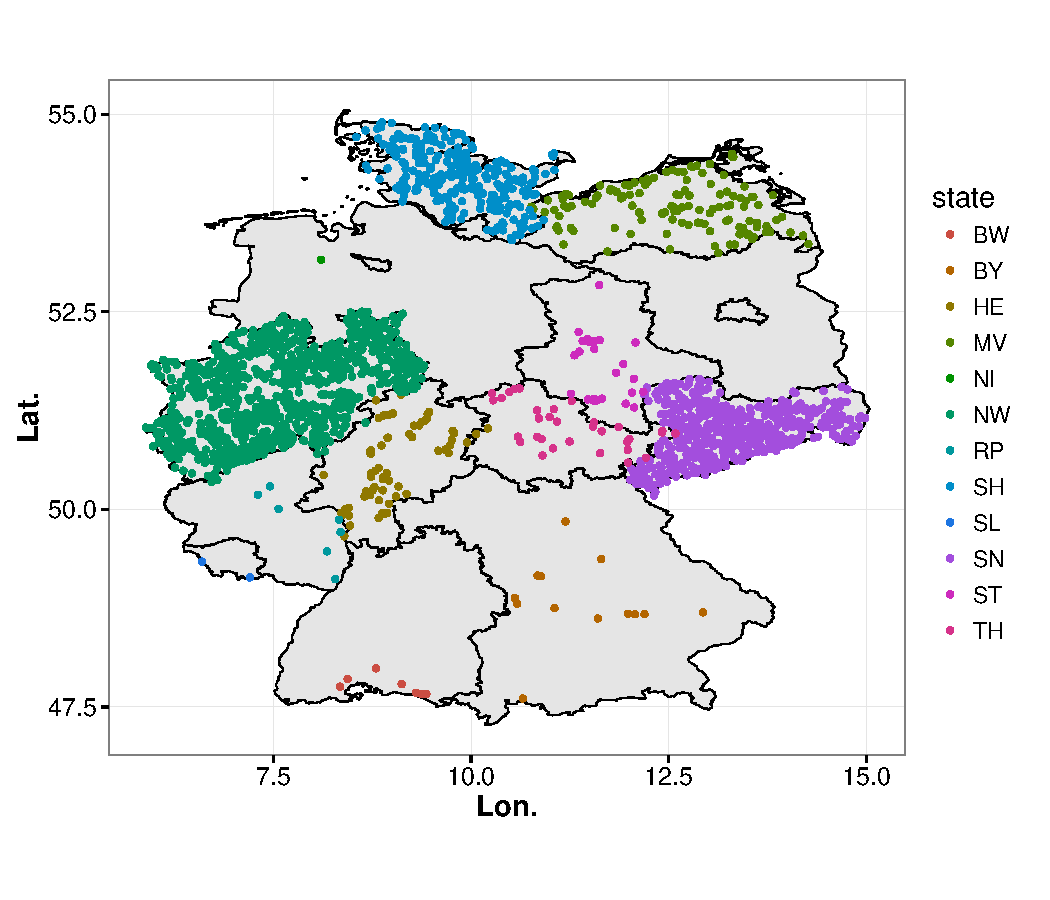
\includegraphics[width=0.6\textwidth]{figure1.pdf}
  \caption{Spatial distribution of the 3109 sampling sites. Colour codes different federal states, see supplemental table S1 for abbreviations.}
  \label{fig:fig1}
\end{figure}

In total 484 different compounds used as pesticides and their metabolites were measured at least once (Supplement, Table S2). 
Most of the compounds were herbicides (179), followed by insecticides (117) and fungicides (109).
Most samples were take in the months April till October, with less samples in the winter (see Supplement, Figure S3).
Only 5.5\% (160,800) of all measurements were detects above the limit of quantification (LOQ).
We found substantial differences in the spectra of analyzed compounds between federal states (Figure \ref{fig:fig2}).
Hierarchical clustering revealed three groups (see also Supplemen,t Figure S4):

\begin{enumerate}[i)]
	\item with less then 100 compounds (SL, ST and TH)
	\item with medium sized spectra
	\item with a big and distinct spectrum (RP and NI)
\end{enumerate}

\begin{figure}[ht]
  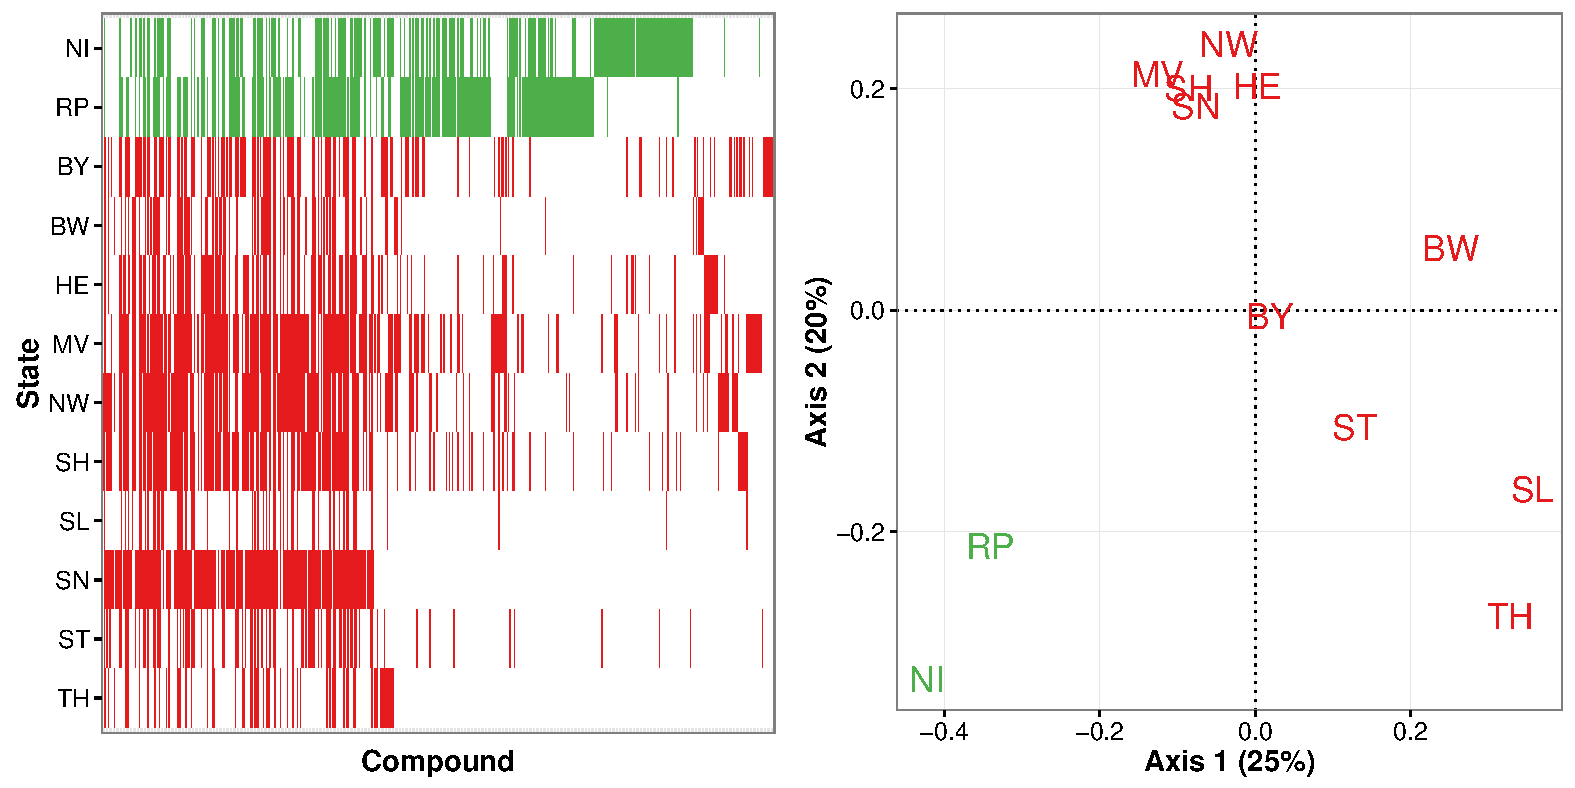
\includegraphics[width=\textwidth]{figure2.pdf}
  \caption{Compound spectra of the different federal states. Left: Barcode plot - each vertical line is an analysed compound. Right: MDS ordination. 
  Colors according to three groups determined by hierarchical clustering (see Supplement, Figure S4).}
  \label{fig:fig2}
\end{figure}

The distribution of sampling sites across catchment area and agricultural area in the catchment revealed a sharp decline in the distribution of catchment-sizes below $10~km^2$, with most sampling sites with catchments between 10 and 25 $km^2$ (Figure \ref{fig:fig3}).
The proportion of agriculture in the catchments decreased with increasing catchment size.

\begin{figure}[ht]
  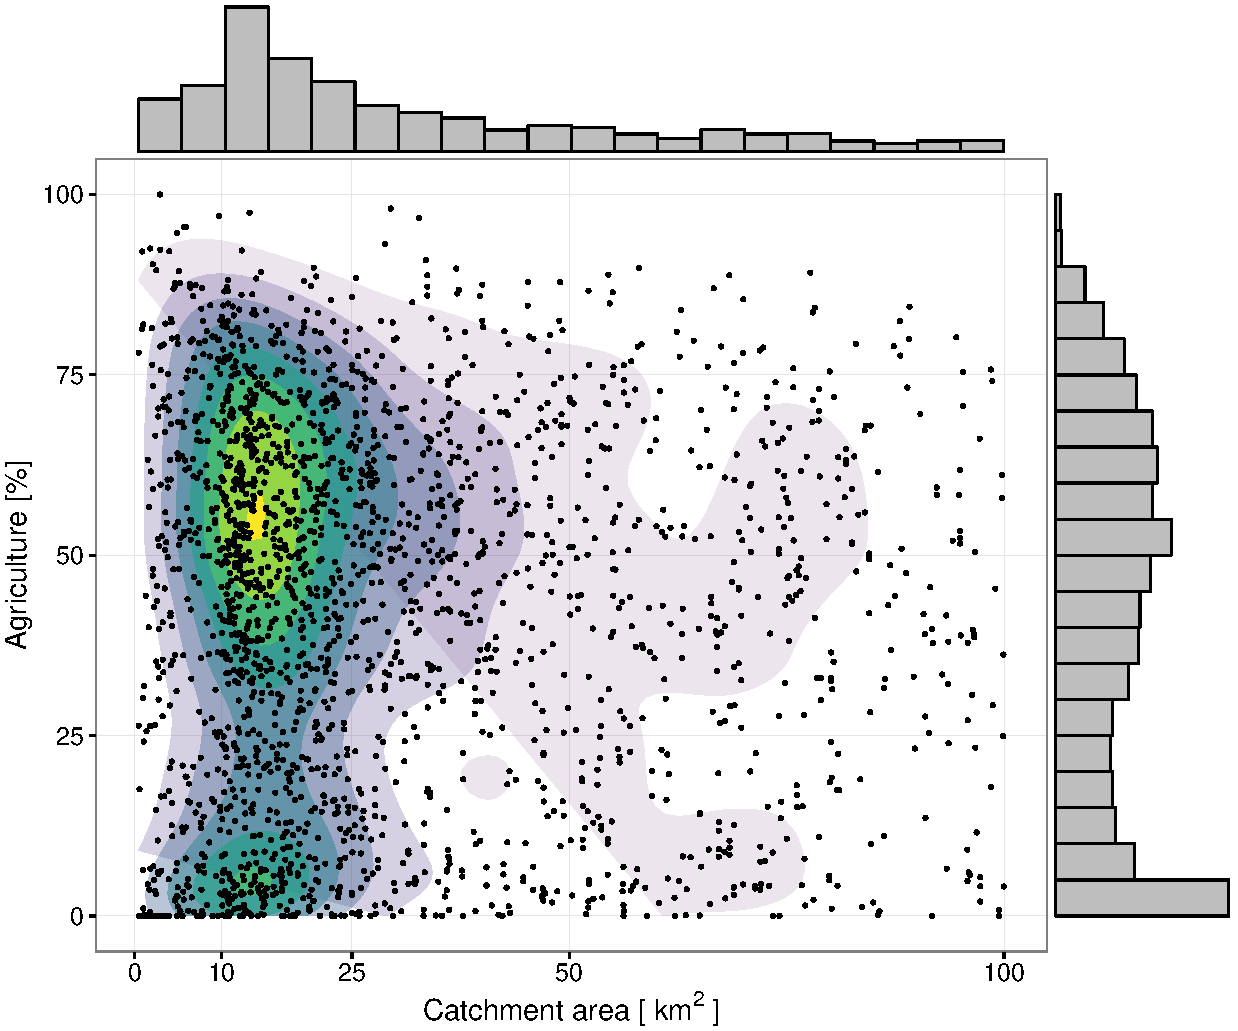
\includegraphics[width=.8\textwidth]{figure3.pdf}
  \caption{Distribution of catchment area and agriculture within the catchment area across the sampling sites.
  Only sampling sites with catchment area < 150 km\textsuperscript{2} are displayed. 
  Colour codes the 2-dimensional density of points.}
  \label{fig:fig3}
\end{figure}


\subsection{Thresholds for agricultural land use and catchment size}
Modeling the number of RAC exceedances as function of agriculture within catchment and catchment size revealed that there is a strong and statistically significant increase up to 25\% agriculture.
Above this threshold the exceedances level off followed by a increase above 75\% (Figure \ref{fig:fig4}, left).
We could no detect any effect of catchment size on the number of RAC exceedances (Figure \ref{fig:fig4}, right).
We also found no statistically significant interaction between catchment size and agriculture.

\begin{figure}[ht]
  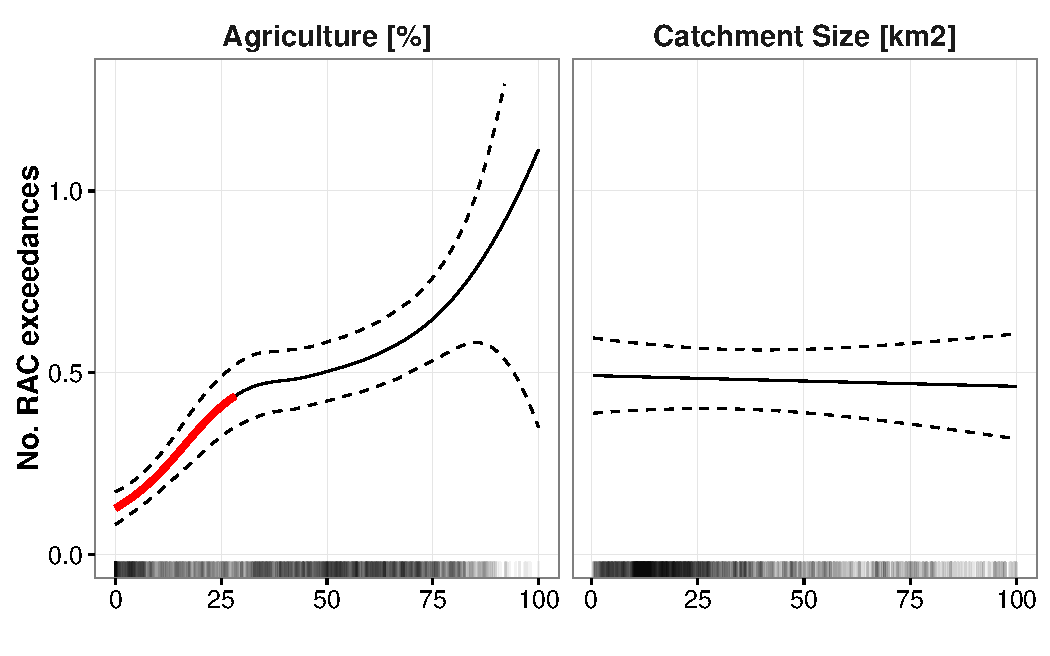
\includegraphics[width=0.95\textwidth]{figure4.pdf}
  \caption{Effect of agriculture within the catchment (left) and catchment size (right) on the number of RAC exceedances. Red line marks statistically significant changes. Dashed lines denote 95\% pointwise Confidence Intervals.
  }
  \label{fig:fig4}
\end{figure}


\subsection{Effect of precipitation on pesticide exposure}
The spatio-temporal intersection revealed that 5\% of the samples were taken at or after days with rainfall events greater than 10mm / day (Supplement, Figure S6).
Precipitation at the day before ($log~precip_{-1}$) sampling increased $\mu$ and also $\pi$ for nearly all analysed compounds. 
The effects were less pronounced ($\pi$) or not clearly directed ($\mu$) for precipitation at the day of sampling ($log~precip_{0}$)(Figure \ref{fig:fig5}, top).

Q2, Q3 and Q4 showed generally higher $\mu$ than in Q1, with smallest differences for Q4.
An exception was the herbicide Diflufenican, that showed througout all quarters lower RQ in Q2-Q4 compared to Q1 (Figure \ref{fig:fig5}, bottom and Supplement Table S4).
We found similar effects of season on $\pi$, but with more compounds showing a reduction in $\pi$.

\begin{figure}[ht]
  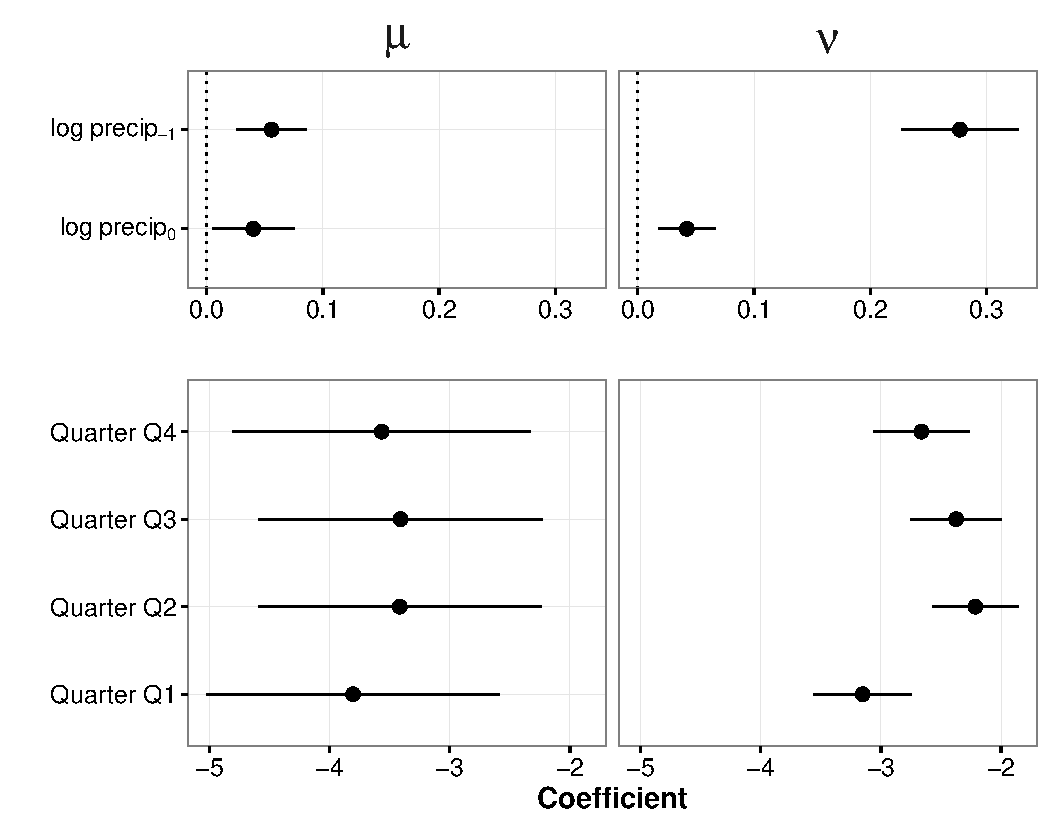
\includegraphics[width=0.95\textwidth]{figure5.pdf}
  \caption{Estimated coefficients and their 95\% CI for the model described in equations \ref{eqn:eqn3} and \ref{eqn:eqn4} for each of the 24 analysed compounds (see Supplement Tables S3 and S4 for a list of compounds from top to bottom and their respective coefficients). Left column: Effect on mean RQ ($\mu$); Right column: effect on the probability that RQ \textgreater 0 ($\pi$).
  Coefficients where the CI encompasses zero are shown in gray colour.
  }
  \label{fig:fig5}
\end{figure}


\subsection{Pesticides in small water bodies}
The dataset comprised 12,710 samples from 1,295 small water bodies.
In 1173 samples (0.3\% of all and 5.6\% of samples with detects) RQ higher then 1 were observed.
Neonicotinoid Insecticides and Chlorpyrifos showed highest risk quotients (Figure \ref{fig:fig6}).
For Thiacloprid, Imidacloprid and Chlorpyrifos RAC was less than LOQ, therefore, all detections have a RQ~\textgreater~1. 
The herbicides Nicosulfuron and Diflufenican, as well as the fungicide Dimoxystrobin also showed high exceedances of RQ (29.5, 14.2 and 21.4 \% of all samples with detects).
Highest RQ were observed for Chlorpyrifos (max(RQ) = 244), Dimoxystrobin(max(RQ) = 117) and Isoproturon (max(RQ) = 80). 
Metabolites were most commonly detected in samples (Metazachlor sulfonic acid was in 82\% of all samples were it was analysed) (Supplement Figure S8).
Glyphosate was the compound with highest detection rates, followed by Boscalid and Isoproturon. 
However, only the latter showed RQ exceedances (Figure \ref{fig:fig6}).
In 44.8\% of samples more then one compound was quantified, with a maximum of 54 different compounds in one samples (Supplement, Figure S7). 

\begin{figure}[ht]
  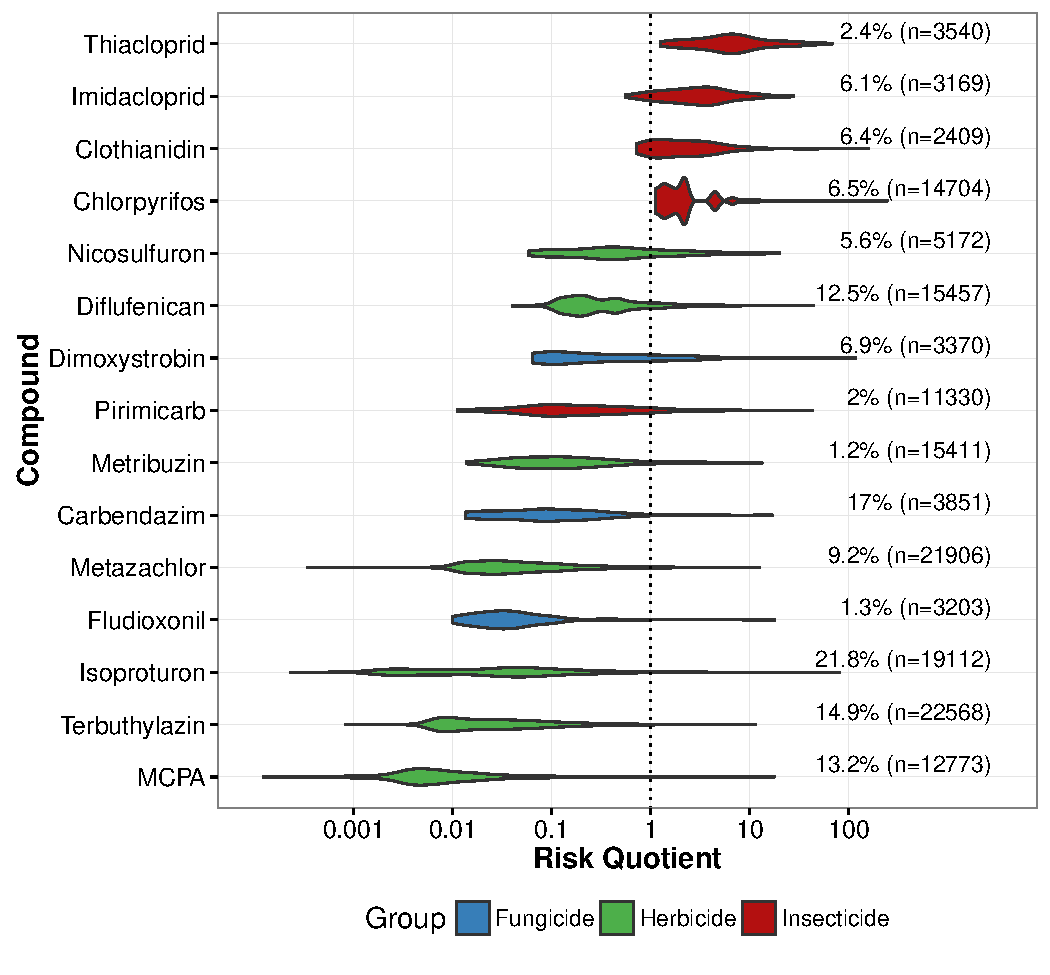
\includegraphics[width=0.6\textwidth]{figure6.pdf}
  \caption{15 compounds with highest risk quotients in SWB. Non-detects are not shown due to the logarithmic axis. Numbers on the right give the percentage of RQ \textgreater 0 and total number of samples.
  }
  \label{fig:fig6}
\end{figure}




%% -------------------------------------------------------------------------
\section{Discussion}
\subsection{Overview on the compiled dataset}
The compiled dataset of governmental monitoring data represents currently the most comprehensive one available for Germany.
Similar nationwide datasets have been compiled for the Netherlands \citep{vijver_spatial_2008}, Switzerland \citep{munz_pestizidmessungen_2011} and the United States (Water Quality Portal (WQP) \url{www.waterqualitydata.us}).
The data compiled and analysed here for Germany is of similar quantity and quality.

% current problems in monitoring and possible solutions
Nevertheless, a nationwide assessment of pesticide pollution is hampered by the inhomogeneity of monitoring data between federal states:
There are not only big differences in the spatial distribution and quantity of sampling sites (Figure \ref{fig:fig1}), but also the spectrum of analyzed compounds (Figure \ref{fig:fig2}) and differences in the quality of chemical analyses. 
For Thiacloprid, Imidaclorpid and Chlorpyrifos LOQ were above RAC.
For these compounds a lowering of LOQ is essential for reliable assessment.
Moreover, would a nation-wide assessment benefit from a harmonized spectrum of analysed compounds.

Given their occurrence in the landscape \citep{nadeau_hydrological_2007} SWB are underrepresented in the current monitoring (Figure \ref{fig:fig3}). 
Especially, streams below 10~km\textsuperscript{2} are missing, which could be attributed to the missing categorisation in the WFD. 



\subsection{Thresholds for agricultural land use and catchment size}
% agriculture
We found a strong influence of agriculture on the pollution of streams.
If there is more the 25\% agriculture within a catchment pesticides it is likely that RAC will be exceeded with an increase in fully agricultural catchments (above 75 \% agriculture).
To our knowledge this is the first study investigating such thresholds of pesticide exposure.
Thresholds for agricultural land use have only been investigated in the past for biological communities.
\citet{feld_response_2013} found change points of biological community metric for agricultural land use at 40\% in low lands. 
Similarly, \citet{waite_agricultural_2014} found a threshold for aquatic diatoms at 40\%.
Our results coincide with these thresholds and suggest that pesticides might contribute to the observed biological changes. 

% size
We did not find a relationship between pesticide pollution and catchment size.
However, previous studies have shown that SWB are more polluted that bigger streams \citep{schulz_field_2004,stehle_pesticide_2015,knauer_pesticides_2016}.
This could be explained by the relatively short gradient of catchment sizes in our dataset, with most of the streams being \textless $100~km^2$ (Figure \ref{fig:fig3}, top).
For example the gradient of \citet{schulz_field_2004} covered 6 orders of magnitude.
Another reason might be the the unequal distribution of catchment sizes, with less sites \textless $10~km^2$ and \textgreater $100~km^2$ (Figure \ref{fig:fig3}, top).



\subsection{Effect of precipitation on pesticide exposure}
Our results revealed that pesticide sampling for chemical monitoring in Germany is mainly performed when no precipitation occurs. 
Nevertheless, we found higher pesticide exposure if samples where taken at the day after heavy rainfall events. 
Interestingly, samples take at they day of the rainfall-event did not show such a strong relationship.
This could be explained by a sampling just before the actual rainfall event.
Pesticide concentration in agricultural SWB show short term peak concentrations \citep{wittmer_significance_2010}, therefore, a sampling at the day after the rain-fall-event might miss peak concentrations.
Overall, our results indicate that current chemical monitoring strongly underestimates pesticide exposure. 
Automatic event-drive samplers \citep{stehle_probabilistic_2013} and passive samplers \citep{fernandez_calibration_2014,moschet_evaluation_2015} may help overcome these shortcomings and provide a better representation, especially for SWB \citep{lorenz_specifics_2016}.

We found pesticide specific patterns in the seasonality of exposure.
Most pesticides showed an increase from April - September, which coincides with their main application season.
Hence, we also found the hightest RQ for the herbicide Diflufenican during the winter/spring season, which is application period for which it is registered in Germany \citep{bvl_online_2016}. 
Our study suggest that pesticide exposure shows compound specific spatio-temporal dynamics.
Currently, little is known on these and further research on those might provide useful information for future ecological risk assessment. 


\subsection{Pesticides in small water bodies}
Our results suggest that SWB are frequently exposed to biologically relevant pesticide concentrations.
\citet{stehle_pesticide_2015} found the highest percentage of RAC exceedances for organophosphate insecticides. 
By contrast, our results revealed that neonicotinoid insecticides show high exceedances, followed by the organophosphate chlorpyrifos. 
This difference can be attributed to the low sample size for neonicotinoid insecticides in their study (n = 33) compared to the dataset presented here (between 1,290 and 2,113 samples in SWB, Figure \ref{fig:fig6}). 
Our results shows that this particular class of insecticides may currently pose a high risk to freshwater ecosystems.
Compared to \citet{stehle_pesticide_2015} we found much lower rates RAC exceedances (0.3\% of 372,304 samples with RAC vs 44\% of 1,566 samples). 
This can be attributed to different aims of the data sources: scientific research aims at finding pollutants, whereas monitoring aims mainly at surveillance of water quality, also during periods with lower pesticide usage and at natural sites. 
Contrary, \citet{knauer_pesticides_2016} found exceedances from monitoring data mainly for herbicides and fungicides and only one insecticide Chlorpyrifos.
This might reflect differences in pesticide use between countries and defined RACs.

From the definition of RAC it follows that if the concentration of a compound exceeds its RAC ecological effects are expected.
Accordingly, \citet{stehle_agricultural_2015} found that biological diversity is significantly reduced at a RQ of 1.12.
We found RQ values greater than 1.12 at 25\% of all SWB sites. 
Consequently, we conclude that pesticides from agricultural land use are a major treat to small water bodies, the biodiversity they host and services they provide. 
Additional treat arises when taking into account that most pesticides do not occur individually but in mixtures \cite{schreiner_pesticide_2016} and may co-occur with other stressors \citep{schafer_contribution_2016}.


% Approval / Risk Assessment
Monitoring data, despite the outlined limitations, provides an opportunity to study large scale environmental occurrences of pesticides.
Nevertheless, such nationwide compilations, may not only be used for governmental surveillance, but also to answer other questions, like validation of exposure modeling \cite{knabel_fungicide_2014}, retrospective evaluation of regulatory risk assessment \citep{knauer_pesticides_2016,stehle_pesticide_2015}or occurrences of pesticide mixtures \cite{schreiner_pesticide_2016}. 
The high exceedances of RAC indicate that the approval process for pesticides must be checked and refined.




%%%%%%%%%%%%%%%%%%%%%%%%%%%%%%%%%%%%%%%%%%%%%%%%%%%%%%%%%%%%%%%%%%%%%
\begin{acknowledgement}
The authors thank the federal state authorities for providing chemical monitoring data and the German Federal Environmental Protection Agency (UBA) for funding a related project (FKZ 3714 67 4040 / 1). 
\end{acknowledgement}


%%% Word count
% abstract    :
% 4 big(600)  : 2400
% 2 small(300): 600
% text body   : 3000 
% ackno       : 24
% ======================================
% total       : 

%%%%%%%%%%%%%%%%%%%%%%%%%%%%%%%%%%%%%%%%%%%%%%%%%%%%%%%%%%%%%%%%%%%%%
\begin{suppinfo}
The following files are available free of charge.
\begin{itemize}
  \item Supplemental\_Materials.pdf : Supplemental Materials (Figures, Tables, Models).
\end{itemize}
\end{suppinfo}


%%%%%%%%%%%%%%%%%%%%%%%%%%%%%%%%%%%%%%%%%%%%%%%%%%%%%%%%%%%%%%%%%%%%%
\bibliography{references}

\end{document}
